\documentclass{easychair}

\title{A note on small explanations\\ for congruence closure}
\titlerunning{A note on congruence closure}

\author{Andreas Fellner\inst{1}
   \and Pascal Fontaine\inst{3}
   \and\\ Georg Hofferek
   \and Bruno Woltzenlogel Paleo
}
\institute{ ****
\and ***
\and Inria, U. of Lorraine (France)}

\authorrunning{Fellner et al.}

\usepackage{amssymb}
\usepackage{graphicx}            			% Figures
\usepackage{tikz}					% tikz graphics
\usetikzlibrary{arrows,automata,positioning}
\usetikzlibrary{fit}
%\usepackage{hyperref}

\newtheorem{example}{Example}
\newtheorem{definition}{Definition}
\newtheorem{corollary}{Corollary}
\newtheorem{theorem}{Theorem}
\newtheorem{lemma}{Lemma}

\begin{document}

\maketitle

\begin{abstract}
The efficiency of Satisfiability Modulo Theories (SMT) solvers is extremely
dependent on the capability of theory reasoners to provide small explanations,
i.e.\ small cores from unsatisfiable sets of input literals.  Decision
procedures for uninterpreted symbols (i.e.\ congruence closure algorithms) date
back from the very early days of SMT.  However, to our best knowledge, the
complexity of small explanation generation for sets of literals with
uninterpreted symbols (and equalities) has never been properly studied.  It is
believed that the small explanation problem for uninterpreted symbols is
NP-complete.  We show here that NP-hardness can indeed be proved using a simple
reduction to SAT.
\end{abstract}


\section*{Introduction}

\section*{Congruence closure}

\section*{NP-completeness of Short Explanation Decision Problem}
\label{sec:npcomplete}

In Section \ref{sec:congruencedef} the notion of explanation is
defined and it is mentioned that we want to find short explanations
in order to compress proofs. In this section we show that the problem
of deciding whether there is an explanation of a given size is NP-
complete, and therefore finding short explanations is hard. Our proof
of NP-completeness reduces the problem of deciding the satisfiability
of a propositional logic formula in conjunctive normal form (SAT) to
the short explanation problem. For basics about satisfiability of
propositional logic formulas and assignments, we refer the reader to
\cite{Biere2009}. We begin by formally defining the problem.


\begin{definition}[Short explanation problem]
Let $E = \{(s_1,t_1),\ldots,(s_n,t_n)\}$ be a set of equations, 
$k \in \mathbb{N}$ and $(s,t)$ be a target equation.  
The \emph{short explanation problem} is the problem of finding 
whether there exists a set $E'$ such that $E' \subseteq E$, 
$E' \models s \thickapprox t$ and $|E'| \leq k$.
\end{definition}

\noindent Our proof of hardness is based on a (polynomial) 
translation of the propositional satisfiability problem to 
the short explanation decision problem.

\newcommand{\Assignment}{{\it Assignment}}
\newcommand{\Clause}{{\it Clause}}
\newcommand{\Connect}{{\it Connect}}

\begin{definition}[CNF Congruence Translation]

Let $\mathcal{C}$ be a set of propositional clauses $\{C_1,\ldots C_n\}$ using variables $x_1,\ldots,x_m$.
%The set of terms $\mathcal{T}$ is constructed using the following constants and function symbols.
%For every $i= 1,\ldots,n + 1$, there is a constant $\hat{c}_i$ and function symbols $t_i$ and $f_i$.
%For every $j= 1,\ldots,m$, there are constants $\hat{x}_j$, $\top_j$ and $\bot_j$.
The congruence translation $E_{\mathcal{C}}$ of $\mathcal{C}$ is defined as the set of equations
\begin{equation*}
\Connect \cup \bigcup_{1 \leq i \leq n}\Clause_i 
\end{equation*}
where
\begin{eqnarray*}
	\Connect &=& \{ (\hat{c}_{i}',\hat{c}_{i+1}) \mid 1 \leq i < n\}\\
        \Clause_i &=& \{ (\hat{c}_i, t_i(\hat{x}_j)) \mid x_j \text{ appears in } C_i \}\\
           & & \cup\ \{ (t_i(\top_j), \hat{c}_i') \mid x_j \text{ appears positively in } C_i \}\\
           & & \cup\ \{ (t_i(\bot_j), \hat{c}_i') \mid x_j \text{ appears negatively in } C_i \}
\end{eqnarray*}

\end{definition}

\noindent This translation is illustrated by the following example.
% and a subset of the translation corresponding to a satisfying assignment.
%We use the standard notion of satisfiability and present variable assignments as sets of those propositional variables being mapped to true.

\begin{example}\label{ex:np1}
Consider the set of clauses $\mathcal{C}$
\begin{equation*}
\big\{C_1 = x_1 \vee x_2 \vee \neg x_3, C_2 = \neg x_2 \vee x_3, C_3 = \neg x_1 \vee \neg x_2\big\}.
\end{equation*}
Figure~\ref{fig:npexamplebig} represents $\Connect \cup \bigcup_{1 \leq i \leq n}\Clause_i$
graphically --- an edge between two nodes meaning that the set contains an
equation between the two nodes --- for the congruence translation $E_{\mathcal{C}}$ of
$\mathcal{C}$.

\begin{figure}[ht]

\centering
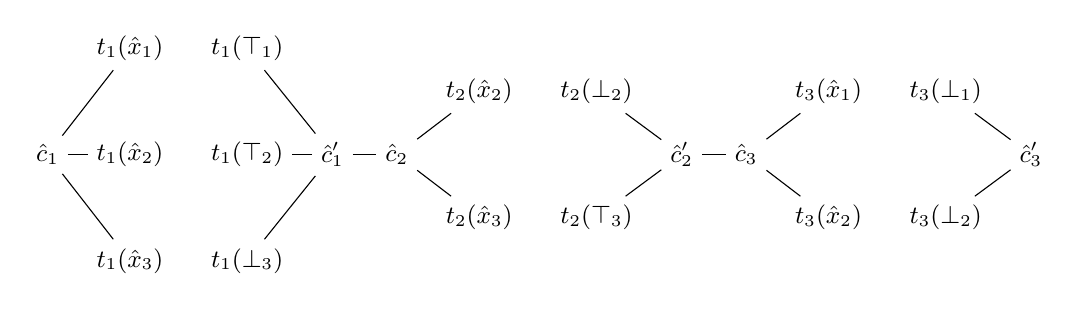
\begin{tikzpicture}[node distance=.3cm]
\small
\node(c1){$\hat{c}_1$};

\node[right =.25cm of c1] (t1x2) {$t_1(\hat{x}_2)$};
\node[above =.8cm of t1x2] (t1x1) {$t_1(\hat{x}_1)$};
\node[below =.8cm of t1x2] (f1x3) {$t_1(\hat{x}_3)$};
\draw [-] (c1) to (t1x2);
\draw [-] (c1) to (t1x1);
\draw [-] (c1) to (f1x3);

\node[right = 3.1cm of c1](c1p){$\hat{c}_1'$};

\node[left =.25cm of c1p] (t12) {$t_1(\top_2)$};
\node[above=.8cm of t12] (t11) {$t_1(\top_1)$};
\node[below=.8cm of t12] (f13) {$t_1(\bot_3)$};
\draw [-] (c1p) to (t11);
\draw [-] (c1p) to (t12);
\draw [-] (c1p) to (f13);

\node[right = .3cm of c1p](c2){$\hat{c}_2$};
\draw [-] (c1p) to (c2);

\node[right=.25cm of c2, yshift=.8cm]  (f2x2) {$t_2(\hat{x}_2)$};
\node[right=.25cm of c2, yshift=-.8cm] (t2x3) {$t_2(\hat{x}_3)$};
\draw [-] (c2) to (f2x2);
\draw [-] (c2) to (t2x3);

\node[right = 3.1cm of c2](c2p){$\hat{c}_2'$};
\node[left =.25cm of c2p, yshift=.8cm]  (f22) {$t_2(\bot_2)$};
\node[left =.25cm of c2p, yshift=-.8cm] (t23) {$t_2(\top_3)$};
\draw [-] (c2p) to (t23);
\draw [-] (c2p) to (f22);

\node[right = .3cm of c2p](c3){$\hat{c}_3$};
\draw [-] (c2p) to (c3);
\node[right =.25cm of c3, yshift=.8cm] (f3x1) {$t_3(\hat{x}_1)$};
\node[right =.25cm of c3, yshift=-.8cm] (f3x2) {$t_3(\hat{x}_2)$};
\draw [-] (c3) to (f3x1);
\draw [-] (c3) to (f3x2);

\node[right = 3.1cm of c3](c3p){$\hat{c}_3'$};
\node[left =.25cm of c3p, yshift=.8cm] (f31) {$t_3(\bot_1)$};
\node[left =.25cm of c3p, yshift=-.8cm] (f32) {$t_3(\bot_2)$};
\draw [-] (c3p) to (f31);
\draw [-] (c3p) to (f32);

\end{tikzpicture}


\caption{$\Connect \cup \bigcup_{1 \leq i \leq n}\Clause_i$}
\label{fig:npexamplebig}
\end{figure}

\end{example}

Assignments can also be translated to sets of equations:
\begin{definition}[Assignment Congruence Translation]
Let $\mathcal{I}$ be an assignment on variables $x_1,\ldots,x_m$.
%The set of terms $\mathcal{T}$ is constructed using the following constants and function symbols.
%For every $i= 1,\ldots,n + 1$, there is a constant $\hat{c}_i$ and function symbols $t_i$ and $f_i$.
%For every $j= 1,\ldots,m$, there are constants $\hat{x}_j$, $\top_j$ and $\bot_j$.
The congruence translation $E_{\mathcal{I}}$ of $\mathcal{I}$ is defined as the set of equations
\begin{eqnarray*}
  E_{\mathcal{I}} & = & \phantom{\cup}\ \{ (\hat{x}_j,\top_j) \mid 1 \leq j \leq m \text{ and } \mathcal{I} \models x_j \} \\
               &   & \cup\ \{ (\hat{x}_j,\bot_j) \mid 1 \leq j \leq m \text{ and } \mathcal{I} \models \neg x_j \}
\end{eqnarray*}
For convenience, we also define the set
\begin{equation*}
  \Assignment^\star = \{ (\hat{x}_j,\top_j), (\hat{x}_j,\bot_j) \mid 1 \leq j \leq m\}.
\end{equation*}
\end{definition}
\noindent
The congruence translation of an assigment is always a subset of the set
$\Assignment^\star$.  By abuse of language, a subset of $\Assignment^\star$ is
said to be an assignment if it is the congruence translation of an assignment,
that is, if it does not contain both $(\hat{x}_j,\top_j)$ and
$(\hat{x}_j,\bot_j)$ for some $j$.

\begin{example}\label{ex:np2} (Example~\ref{ex:np1} continued).\\
Consider the model $\mathcal{I} = \{x_1, \neg x_2, x_3\}$ of $\mathcal{C}$.
Figure~\ref{fig:npassignment} gives a graphical representation of
$E_{\mathcal{I}}$, whereas $\Assignment^\star$ is described by
Figure~\ref{fig:npassignmentstar}.  Notice that
$E_{\mathcal{C}} \cup E_{\mathcal{I}} \models \hat{c}_1 = \hat{c}'_3$,
and $\hat{c}_1$ and $\hat{c}'_3$ are connected in the congruence graph\marginpar{congruence graph: define}
of $E_{\mathcal{C}} \cup E_{\mathcal{I}}$ (Figure~\ref{fig:npmodel}).
This is actually the aim of the construction.

\begin{figure}[ht]

\centering
\begin{tikzpicture}[node distance=1.5cm]

\node [below =.5cm of f2x2] (x1) {$\hat{x}_1$};
\node [below =.5cm of x1] (x2) {$\hat{x}_2$};
\node [below =.5cm of x2] (x3) {$\hat{x}_3$};

\node [right = of x1] (t1) {$\top_1$};

\draw [-] (x1) to (t1);

\node [left = of x2] (f2) {$\bot_2$};

\draw [-] (x2) to (f2);

\node [right = of x3] (t3) {$\top_3$};

\draw [-] (x3) to (t3);

\end{tikzpicture}


\caption{Congruence translation of $\mathcal{I}$}
\label{fig:npassignment}
\end{figure}

\begin{figure}[ht]

\centering
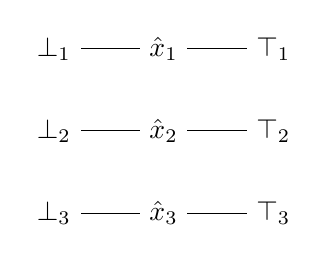
\begin{tikzpicture}[node distance=.75cm]

\node (x1) {$\hat{x}_1$};
\node [below =.5cm of x1] (x2) {$\hat{x}_2$};
\node [below =.5cm of x2] (x3) {$\hat{x}_3$};

\node [right = of x1] (t1) {$\top_1$};
\node [left = of x1] (f1) {$\bot_1$};

\draw [-] (x1) to (t1);
\draw [-] (x1) to (f1);

\node [right = of x2] (t2) {$\top_2$};
\node [left = of x2] (f2) {$\bot_2$};

\draw [-] (x2) to (t2);
\draw [-] (x2) to (f2);

\node [right = of x3] (t3) {$\top_3$};
\node [left = of x3] (f3) {$\bot_3$};

\draw [-] (x3) to (t3);
\draw [-] (x3) to (f3);

\end{tikzpicture}



\caption{$\Assignment^\star$}
\label{fig:npassignmentstar}
\end{figure}
\begin{figure}[ht]

\centering
\begin{tikzpicture}[node distance=.3cm]
\small
\node(c1){$\hat{c}_1$};

\node[right =.25cm of c1] (t1x2) {$t_1(\hat{x}_2)$};
\node[above =.8cm of t1x2] (t1x1) {$t_1(\hat{x}_1)$};
\node[below =.8cm of t1x2] (t1x3) {$t_1(\hat{x}_3)$};
\draw [-] (c1) to (t1x2);
\draw [-] (c1) to (t1x1);
\draw [-] (c1) to (t1x3);

\node[right = 3.1cm of c1](c1p){$\hat{c}_1'$};

\node[left =.25cm of c1p] (t12) {$t_1(\top_2)$};
\node[above=.8cm of t12] (t11) {$t_1(\top_1)$};
\node[below=.8cm of t12] (t13) {$t_1(\bot_3)$};
\draw [-] (c1p) to (t11);
\draw [-] (c1p) to (t12);
\draw [-] (c1p) to (t13);

\node[right = .3cm of c1p](c2){$\hat{c}_2$};
\draw [-] (c1p) to (c2);

\node[right=.25cm of c2, yshift=.8cm]  (t2x2) {$t_2(\hat{x}_2)$};
\node[right=.25cm of c2, yshift=-.8cm] (t2x3) {$t_2(\hat{x}_3)$};
\draw [-] (c2) to (t2x2);
\draw [-] (c2) to (t2x3);

\node[right = 3.1cm of c2](c2p){$\hat{c}_2'$};
\node[left =.25cm of c2p, yshift=.8cm]  (t22) {$t_2(\bot_2)$};
\node[left =.25cm of c2p, yshift=-.8cm] (t23) {$t_2(\top_3)$};
\draw [-] (c2p) to (t23);
\draw [-] (c2p) to (t22);

\node[right = .3cm of c2p](c3){$\hat{c}_3$};
\draw [-] (c2p) to (c3);
\node[right =.25cm of c3, yshift=.8cm] (t3x1) {$t_3(\hat{x}_1)$};
\node[right =.25cm of c3, yshift=-.8cm] (t3x2) {$t_3(\hat{x}_2)$};
\draw [-] (c3) to (t3x1);
\draw [-] (c3) to (t3x2);

\node[right = 3.1cm of c3](c3p){$\hat{c}_3'$};
\node[left =.25cm of c3p, yshift=.8cm] (t31) {$t_3(\bot_1)$};
\node[left =.25cm of c3p, yshift=-.8cm] (t32) {$t_3(\bot_2)$};
\draw [-] (c3p) to (t31);
\draw [-] (c3p) to (t32);

\node [below =1.3cm of c2, xshift=1.5cm] (x1) {$\hat{x}_1$};
\node [below =.5cm of x1] (x2) {$\hat{x}_2$};
\node [below =.5cm of x2] (x3) {$\hat{x}_3$};

\node [right = of x1] (t1) {$\top_1$};

\draw [-] (x1) to (t1);

\node [left = of x2] (t2) {$\bot_2$};

\draw [-] (x2) to (t2);

\node [right = of x3] (t3) {$\top_3$};

\draw [-] (x3) to (t3);

\draw [dotted] (t1x1) to (t11);
\draw [dotted] (t1x3) to (t13);
\draw [dotted] (t2x2) to (t22);
\draw [dotted] (t2x3) to (t23);
\draw [dotted] (t3x2) to (t32);

\end{tikzpicture}


\caption{The congruence graph for $E_{\mathcal{C}} \cup E_{\mathcal{I}}$}
\label{fig:npmodel}
\end{figure}
\end{example}

\begin{lemma}
\label{lemma:eqv}
Consider a (partial or total) assignment $\mathcal{I}$ for a set of clauses
$\mathcal{C}= \{C_1, \dots C_n\}$.  $\mathcal{I} \models \mathcal{C}$ if and only if
$E_{\mathcal{I}} \cup E_\mathcal{C} \models \hat{c}_1 \thickapprox \hat{c}'_n$.
\end{lemma}
\begin{proof}
The condition is sufficient.  Consider the congruence graph induced by
$E_{\mathcal{I}} \cup E_\mathcal{C}$.  Besides edges directly associated to
equalities in the set, the only edges are congruence edges between terms
$t_i(\hat{x}_j)$ and either $t_i(\top_j)$ or $t_i(\bot_j)$.  So any path from
$\hat{c}_1$ to $\hat{c}_n$ would go through such a congruence edge for each $i$.
And such an edge exist for $i$ if and only if clause $i$ is satisfied by
$\mathcal{I}$.

The condition is also necessary.  If $\mathcal{I} \models \mathcal{C}$, then
$\mathcal{I} \models C_i$ for each clause $C_i \in \mathcal{C}$.  Assume
$\mathcal{I}$ makes true a variable $x_j$, literal of $C_i$ (the case of
negation of a variable is handled similarly).  Then $E_{\mathcal{I}} \models
t_i(\hat{x}_j) \thickapprox t_i(\top_j)$, and $E_{\mathcal{I}} \cup \Clause_i
\models \hat{c}_i \thickapprox \hat{c}_i'$.  This is true for each $i$, and
thanks to the equations in \Connect, one can deduce using transitivity that
$E_{\mathcal{I}} \cup E_\mathcal{C} \models \hat{c}_1 \thickapprox \hat{c}_n'$.
\end{proof}

\noindent Notice also that, for any model $\mathcal{I}$ of a set of $n$ clauses
$\mathcal{C}$, every explanation that $E_{\mathcal{I}} \cup E_\mathcal{C}
\models \hat{c}_1 \thickapprox \hat{c}_n'$ contains at least two equalities in
each set $\Clause_i$, since each clause has to be satisfied.  But also, there is
an explanation that contains exactly two equalities in each set $\Clause_i$.
Considering again Example~\ref{ex:np2}, and particularly
Figure~\ref{fig:npmodel}, any transitivity chain from $\hat{c}_1$ to
$\hat{c}'_3$ will pass through $\hat{c}'_1$, $\hat{c}_2$, $\hat{c}_2'$ and
$\hat{c}_3$.  Any acyclic path from $\hat{c}_1$ to $\hat{c}'_3$ will contain 11
edges: 3 congruence edges, $3\times 2$ edges in $\Clause_i$ for $i=1,\dots 3$
and 2 edges from $\Connect$.

Since every interpretation $\mathcal{I}$ is such that $E_{\mathcal{I}} \subset
\Assignment^\star$, one can try to relate the propositional satisfiability
problem for a set of clauses $\mathcal{C}= \{C_1, \dots C_n\}$ to finding an
explanation of $\hat{c}_1 \thickapprox \hat{c}_n'$ in $\Assignment^\star \cup
E_{\mathcal{C}}$.  However, it is necessary that this explanation does not set
$\hat{x}_j$ equal both to $\top_j$ and $\bot_j$, i.e.\ at most one of the two
equations $(\hat{x}_j,\top_j)$ and $(\hat{x}_j,\bot_j)$ should be in the
explanation.  By restricting assignments to total ones, i.e.\ by enforcing that
at least one of the two equations $(\hat{x}_j,\top_j)$ and $(\hat{x}_j,\bot_j)$
belongs to the explanation, it is also possible, with a single cardinality
constraint on the explanation, to require that at most one of them belong to the
explanation.

\marginpar{Bruno: There seems to be redundancy between the informal paragraph above and the formal proof below. The paragraph seems more formal and detailed than necessary, while the proof perhaps less detailed than necessary.}

\begin{lemma}
A set of clauses $\mathcal{C}= \{C_1, \dots C_n\}$ using variables $x_1,\dots
x_m$ is satisfiable if and only if there is a subset $E' \subseteq
\Assignment^\star \cup E_{\mathcal{C}'}$ such that $E'\models \hat{c}_1
\thickapprox \hat{c}'_{n+m}$ and $|E'| \leq 3n+4m-1$, where $\mathcal{C}'$ is
$\mathcal{C}$ augmented with the tautological clauses $c_{n+i} = x_i \vee \neg
x_i$ for $i=1,\dots m$.
\end{lemma}
\begin{proof}
The condition is straightforwardly necessary.  It is also sufficient since an
explanation of $\hat{c}_1 \thickapprox \hat{c}'_{n+m}$ has to contain $2(n + m)$
equations from $Clause_i$ ($i= 1\dots n + m$) and $n + m - 1$ equations from
$\Connect$.  Thanks to the tautological clauses, any explanation also has to
contain at least $(\hat{x}_j,\top_j)$ or $(\hat{x}_j,\bot_j)$ for each
$j\in\{1\dots m\}$. Therefore, the cardinality constraint requires that the explanation
contain at most one $(\hat{x}_j,\top_j)$ or $(\hat{x}_j,\bot_j)$ for each
$j\in\{1\dots m\}$.  If such an explanation exists, Lemma~\ref{lemma:eqv}
guarantees the existence of a model for $\mathcal{C'}$, or equivalently for
$\mathcal{C}$.
\end{proof}




\begin{corollary}[NP-hardness]
\label{lemma:nphardness}
The short explanation decision problem is NP-hard.
\end{corollary}

\begin{lemma}[NP]
\label{lemma:innp}
The short explanation decision problem is in NP.
\end{lemma}
\begin{proof}
Explanations are subsets of the input equations, therefore they are clearly
polynomial in the problem size.  The congruence of two terms, i.e. verifying
that a subset is actually an explanation, can be decided in polynomial
time\marginpar{be more precise}\marginpar{bruno:citation needed?} using classical congruence closure algorithms.
\end{proof}

Lemmas~\ref{lemma:nphardness} and~\ref{lemma:innp} thus establish:

\begin{theorem}[NP-completeness]
The short explanation decision problem is NP-complete.
\end{theorem}

\section*{Conclusion}


\end{document}
